\section{RELATED WORKS}
    Exploring the state of the art of alternatives of height sensoring, new approaches based on the use of images show great potential for identifying the distances between vehicle and surface as seen in artificial intelligence techniques both using neural networks \cite{MonocularDepth} \cite{Joglekar2011DepthEU}, or traditional algorithm-based and hardware-based options with numerical enhancements and optimizations in target detection and tracking operations \cite{SurveyObjDetectionTracking}, obstacle avoidance \cite{CNNSingleImageQuadrotor} \cite{AircraftColAvoid}, navigation \cite{ByMySelf}, among others \cite{OpticalFlowStereo}.
    To this end, the use of real-time operation technologies such as MobileNet can be considered, offering adequate performance with low latency and low power consumption, so desired in autonomous mobile robotics applications \cite{MobileNetTracking}.
    
    The field of work about applications with sparse image banks relies on the aid of synthetic images, or modified with elements of real or synthetically generated cut-outs, in order to simulate the desired situations \cite{BlenderSmoke} \cite{BlurFiducial} \cite{ObjetoSintetico} \cite{TurbineBlur} \cite{BlenderMapa}.
    Initially the process can use much time that could be oriented to experiments, but this allow a safer use of field equipment, especially in proof-of-concept and testing stages, by not requiring the use of materials, often difficult to access and with a considerable budget. 
    At the same time, these methods are able to show how accurate the results of predictions and calculations based on the sets manipulated with software tools can be. 
    Moreover, human capital is also saved, dispensing with operators in unhealthy environments. 
    Bringing the discussion to the present scenario, UAV operators would need a hitherto unjustified sun exposure to capture a long image bank without knowing the prediction capability of neural network systems. 
    In the past few years, artificial intelligence technology and computer vision technology have been expanding rapidly.
    
    \subsection{CNN Based UAVs Estimations}
    Currently, the available technologies for altitude estimation for unmanned aerial vehicles are mainly based on traditional algorithms, with linear processing of data from barometers, ultrasound, and Light Detection and Ranging (LiDAR) \cite{MonocularDepth}. 
    Such methods have particularities with advantages and disadvantages particular to each technology, making it unfeasible to use them in all and any situations, requiring considerations in applying them according to the terrain, weather conditions, altitude of intended operation, currently lacking a complete method capable of meeting the demands of a generalist way \cite{FiltroKalmanAltitude}. 
    Even using modern sensor fusion filters, some scenarios are still infeasible for autonomous operation, such as highly reflective surfaces found in dunes, snow, and water \cite{WeatherConstraints}.
    
    Therefore, it is reasonable to believe that CNNs can also promote the development of height estimation.
    And, recently, some works can present convincing capabilities to use CNNs in this subject. 

    \cite{OnboardCNN} proposed a CNN for Single Shot Detection with seven layers (SSD7) for identifying landing conditions running along with ROS in a low power Intel Stick M3, reaching 13 fps in real time. 

    \cite{ByMySelf} trained a CNN for a self-supervised UAV to fly indoors, recognizing distances on camera, avoiding obstacles, and navigating autonomously. RGB images were processed with IR and ultrasonic data in a parallel input model based on AlexNet. The system has as output, the prediction of a set of options with associated direction and speed to avoid collisions and navigate safely.

    \cite{MobileNetTracking} proposed a model for light-weight UAV object tracking, with distance calculation, aiming the real time operation in low power mobile devices.
    The architecture chosen was based on MobileNet and his variants, MobileNetv1, MobileNetv2 and E-MobileNet with 7 hidden-layers, reaching 56fps running on a NVIDIA Jetson AGX Xavier, with average accuracy of 87,2\%.
    
    \subsection{Training With Synthetic Generated Data Sets}
    
    This strategy is an increasingly widespread practice in case studies with sparse, and costly to produce in-house, real image banks.
    Currently there are no open image banks under the conditions desired for this work, consisting of cameras pointing at the water surface perpendicularly associated with height and/or other odometry data, so modeling and rendering a photorealistic water surface has become a necessity.

    Among related work using this strategy, depending on the purpose, montages can be made using partially real and partially computer-generated images for the inclusion of elements.
    In the present case, and current stage of development, partially fit real images would only be useful for manipulation with the removal of elements, if, for example, there were banks with the above characteristics, but contaminated by undesired elements, such as marine life, garbage, and boats.
    Image reconstruction strategies may be considered in the future.
    
    \cite{TurbineBlur} considered the effects of motion blur in image capture of wind turbine systems, monitored by UAVs.
    Adequate and quality cataloged images are not available for this application, and the integrity of the measurements impacts the health diagnosis of the wind blades.
    The solutions found are based on capturing clear images of stationary turbines and combining three strategies, including the use of generative hybrid networks.
    For the first procedure, images of moving propellers were combined with images of the same stopped propellers.
    The second method dealt with manipulating these images with motion blur by means of a generative network fed with real images of distorted turbines to form a hybrid network of distorted images.
    In the third method, the movements of the propellers were simulated in order to extract parameters used for the production of virtually blurred images.
    After the images were produced, the bank was restored by another network and tested with a network model proposed by the researcher, called M-DeblurGANv2 and based on an already established network used for distorted image treatments, the DeblurGAN.
    The surface diagram of all processing steps is shown in the Figure. \ref{fig:TurbinaDiagrama}.
    
    \begin{figure}[!h]
        \centering 
        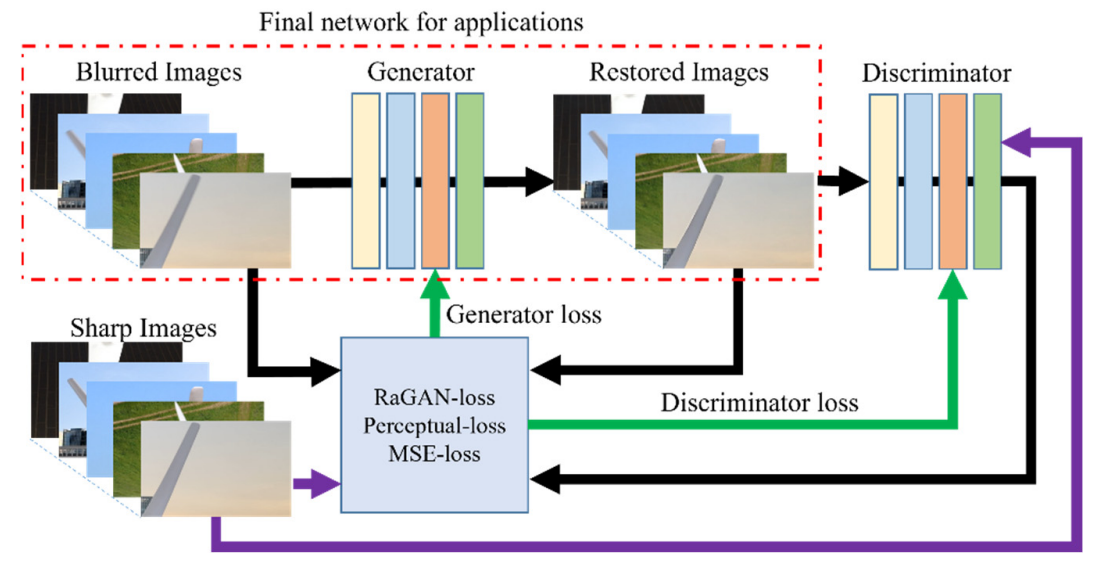
\includegraphics[width=15cm]{Images/turbinablur.png}
        \caption{Flowchart of DeblurGANv2-based motion deblurring of wind turbine blade images. \cite{TurbineBlur}}
        \label{fig:TurbinaDiagrama}
    \end{figure}
    
    \cite{BlenderSmoke} used a Faster R-CNN network to detect smoke from forest fires, aiming to eliminate the problems of manual detection and extraction of images by conventional methods. 
    However, suitable forest smoke images are sparse, making it impossible to train robust neural networks with low sampling, given the limits of scaleless sparse data augmentation and diversity.
    The way out the researchers found was to generate two synthetic banks. 
    Synthetic smoke was added to videos of non-fire landscapes, and for this, the techniques chosen were:
    \begin{itemize}
	    \item with a real smoke on a green background inside a studio;
    	\item rendering of fictitious smoke by Blender.
    \end{itemize}
    The results were crossed, between the trained model with the image bank added to the real smoke, and the bank added to the images rendered by Blender, with great results, with advantage for the set of images edited with synthetic smoke.
    
    \cite{ObjetoSintetico} worked on the problem of filling the need for a large cataloged image bank for training needs. The main objects of the research were food packages in refrigerators, with only real images available from the internet. The banks were divided as follows: Real bank with 400 real images, fully synthetic bank with 4000 images rendered in Blender, and a hybrid bank disposing of 3600 synthetic images and the 400 real images.
    The network chosen for training was GoogleNet Fully Convolutional, in 200 epochs, with various mixed techniques of early stopping and layer-specific fine-tuning.
    Finally, the result of the work converged to a mAP (mean average precision) of 24 for the system trained with synthetic images only, 28 for the system with real images only, and 36 for the mixed system.

    \cite{BlenderMapa} created three-dimensional environments in Blender, aiming to freely generate image samples in distinct poses to emulate the manipulation of mobile devices.
    The goal was to reconstruct the pose and location based on the features of the environment.
    It was possible to train a PoseNet network, based on GoogLeNet of 23 layers and six inception modules to achieve an accuracy of about 2m in real time.
    
    
    %\subsection{Resume}
    
    %The advantages of all the methodological base used in this work are evident, allowing a gradual employment of resources, whether hardware, software or human, with the leveling of working conditions at each step, bringing an efficient sequence of construction versed in adaptability. 
    %Therefore, by making use of these relationships, it is possible to explore a new approach to extracting features from images and composing increasingly refined sensor filters using conventional cameras, already present in UAVs, with only the addition of parallelizing a low-energy software process \cite{MobileNetTracking}.